% !TeX spellcheck = en_GB
% !TeX root = ReportMain.tex
%\section{Electrical Breakdown in High Voltage Systems} %Possibly a better heading needed
\section{Overview of Insulation Failure Modes\todo{is this a better name?}}
There are some consequences that need to be taken into account when designing systems for operation at high voltage. 
High voltage systems generate a higher electric potential than surrounding objects, which are usually at earth potential. 
These arise large electric potential gradients or electric fields. 
The values of high field regions within the electric field may cause electrical breakdown and partial discharges leading to failure of the system \citep{kuffel2000high}. 
It is therefore important to design systems to minimise the chance of these events.\todo{figure ref}

\begin{figure}[!h]
   \centering
   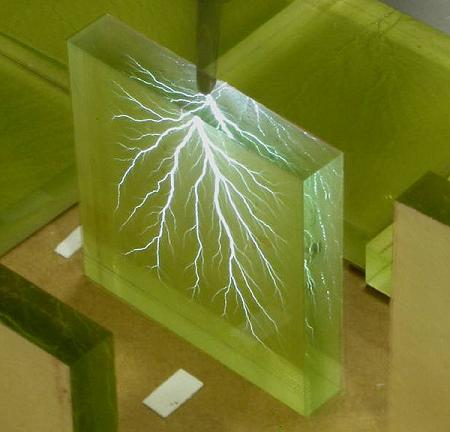
\includegraphics[width = 0.5\textwidth]{lichtenberg-figures004.jpg}
   \caption{Electrical tree tracing the path of damaged insulation caused by electrical breakdown}
   \label{figure:breakdown}
\end{figure}
%http://damnamazing.blogspot.co.uk/2008/11/captured-lightning-lichtenberg-figures.html

Electrical breakdown is the action of electrical conduction across an insulating medium, usually a dielectric, following the voltage across this medium exceeding the breakdown voltage of the specific material. 
This usually happens when the potential difference is extremely high and arcing can be seen in gaseous insulating mediums. 
This can cause changes to the compounds in the insulating medium and also cause damage to equipment in the form of treeing as shown in figure \ref{figure:breakdown}. 

There are different types of electrical breakdown to consider. 
The main types of electrical breakdown that are involved in high voltage insulation systems are general breakdown in the system, surface flashover, partial discharge in the dielectric insulation as well as corona discharge in air.

\subsection{General Breakdown \todo{Is this intrinsic breakdown}}  %intrinsic? - cite kuffel
In the case of a high voltage transformer bushing, there is a combination of both high electric fields and a close proximity to the grounded surroundings. 
As mentioned in section \ref{s:into}, the purpose of a bushing is to insulate the conductor from ground. 
The most basic form of bushing is a non-condenser bushing \cite{HVEngandTesting}. 
It is the radial component of the tangential electric field that causes this typical breakdown directly from the conductor to the grounded flange. 
Insulation must have a very high dielectric constant to withstand high voltage conditions.
Typical materials used for bushing manufacture include Resin-impregnated paper (RIP) and Oil-impregnated paper (OIP). 
The importance of this type of bushing is that as the electric strength of the insulation increases, radial thickness may be reduced \cite{HVEngandTesting}. 
Typically the general breakdown strength of bushings is very high relative to PD inception and is only a secondary concern.

\subsection{Surface Flashover}
The partnering electric breakdown effect for solid, non-condenser bushing is surface flashover; breakdown caused by the electric field travelling from the conductor to the surroundings via the surface of the bushing. 
The properties governing the axial height of the bushing are both the axial electric field and the surrounding medium \cite{HVEngandTesting}.
Typically the criteria for surface flashover breakdown is much lower than general breakdown, and improvements to the bushing have primarily been in shaping the axial field distribution. 
This investigation considers an air-to-oil bushing and as oil is more than twice as strong dielectrically as air at atmospheric pressure the air end must be approximately twice as long \cite{harlow2004electric}.
Creepage distance is a critical factor here, as defined in the IEC 60137 standard as the ``shortest distance along the surface of an insulator between two conductive parts'' \cite{IEC60137}.
For industrial standard bushings, ceramic shedding is used to extend the length of the surface of the bushing. 
While this is beyond the scope of this report and therefore not modelled, it is important to note that it will typically increase the effective axial length of the bushing by a factor of 4.

\subsection{Partial Discharge}
Partial Discharge (PD) is defined by the British Standards 60270:2001 as a “localized electrical discharge that only partially bridges the insulation between conductors and which can, or can not, occur adjacent to a conductor” and as “a consequence of local electrical stress concentrations in the insulation” \cite{60270}. 
The most common cause of partial discharge is a void, originating from manufacturing imperfections, within the dielectric material where the void contains material of a lower electrical breakdown strength (gas or air) than the dielectric material. 
Under high electric fields across the dielectric insulation these voids will experience local electrical breakdown as the rate of charge increase is greater than decay and inception voltage is exceeded. 
Due to these conditions, PDs typically occur under intense tangential electric field resulting in electron emission \cite{surfaceflashover} and as the discharges spread across the surface of the solid dielectric breakdown will occur \cite{kuffel2000high}. In order to ensure the insulation system can sufficiently reduce the chance of PD, the inception voltage of the insulation must be relatively high compare to the operating voltage of the conductor.

Partial discharge is a primary cause of ageing within High Voltage systems, this is because each successive discharge applies electro-mechanical forces to the void itself and the insulation progressively deteriorates \cite{PDageing}. Therefore reducing tangential electric fields and measurement of PDs is of high importance. 

\subsection{Corona Discharge}
Corona discharge is the ionisation of fluid around a conductor of high electric potential. The ionisation of the surrounding fluid is due to the discharge from the conductor. In high voltage systems, corona discharge occurs most commonly from the conductor to air surrounding the conductor as illustrated in figure \ref{figure:corona}. Corona discharge occurs at an area of intense electric field, but not sufficiently intense to cause arcing. This type of breakdown might not cause fatal damage to the insulation, but would shorten the life time of the insulation system. It also represents power losses to the surrounding, so it is important to design insulation system minimising the effect of corona discharge. \todo{References in text and figure}

\begin{figure}[!h]
   \centering
   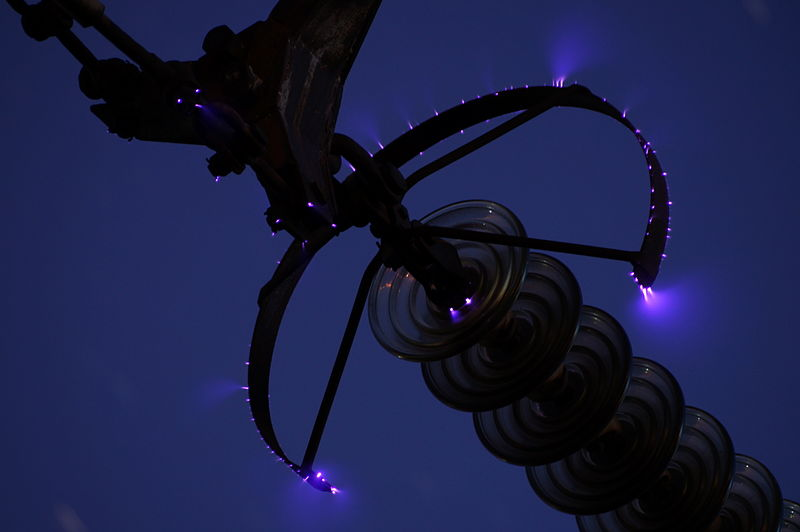
\includegraphics[width = 0.5\textwidth]{coronadischarge.jpg}
   \caption{Corona discharge appearing on the insulation surface of high voltage conductor}
   \label{figure:corona}
\end{figure}
%Problem, this picture is from wikipedia